\documentclass[10pt,aspectratio=43,mathserif,table]{beamer} 
%  设置为 Beamer 文档类型,设置字体为 10pt,长宽比为16:9,数学字体为 serif 风格
\batchmode

\usepackage{graphicx}
\usepackage{animate}
\usepackage{hyperref}
\usepackage{diagbox} % 表头斜线分区
% 导入一些用到的宏包
\usepackage{amsmath,bm,amsfonts,amssymb,enumerate,epsfig,bbm,calc,color,ifthen,capt-of,multimedia,hyperref}
\usefonttheme{serif}
\usepackage{mathptmx}
\usepackage{xeCJK} %导入中文包
%\setCJKmainfont{SimHei} %字体采用黑体  Microsoft YaHei
%\setmonofont{Courier New}
%\setCJKmainfont[AutoFakeBold = {2.15},ItalicFont={KaiTi}]{SimSun}
%\setCJKfamilyfont{xw}{STXinwei}

%\setsansfont{Microsoft YaHei}

%\setsansfont{Arial}


\usetheme{Berlin} %主题
%\usecolortheme{sustech} %主题颜色

\usepackage[ruled,linesnumbered]{algorithm2e}

\usepackage{fancybox}
\usepackage{xcolor}
% \usepackage{times}
\usepackage{listings}

\usepackage{booktabs}
\usepackage{colortbl}

\newcommand{\Console}{Console}
\lstset{ %
	backgroundcolor=\color{white},   % choose the background color
	basicstyle=\footnotesize\rmfamily,     % size of fonts used for the code
	columns=fullflexible,
	breaklines=true,                 % automatic line breaking only at whitespace
	captionpos=b,                    % sets the caption-position to bottom
	tabsize=4,
	commentstyle=\color{mygreen},    % comment style
	escapeinside={\%*}{*)},          % if you want to add LaTeX within your code
	keywordstyle=\color{blue},       % keyword style
	stringstyle=\color{mymauve}\ttfamily,     % string literal style
	numbers=left, 
	%	frame=single,
	rulesepcolor=\color{red!20!green!20!blue!20},
	% identifierstyle=\color{red},
	language=c
}


\definecolor{mygreen}{rgb}{0,0.6,0}
\definecolor{mymauve}{rgb}{0.58,0,0.82}
\definecolor{mygray}{gray}{.9}
\definecolor{mypink}{rgb}{.99,.91,.95}
\definecolor{mycyan}{cmyk}{.3,0,0,0}

%题目,作者,学校,日期
\title{Ising model}
%\subtitle{\fontsize{9pt}{14pt}\textbf{跨临界分岔}}
\author{Speaker: Yichen Lu\quad \newline  \newline \quad }
\institute{\fontsize{8pt}{14pt}}
\date{\today}
\newcommand{\concept}{Ising model}

%学校Logo
%\pgfdeclareimage[height=0.5cm]{sustech-logo}{sustech-logo.pdf}
%\logo{\pgfuseimage{sustech-logo}\hspace*{0.3cm}}

\AtBeginSection[]
{
	\begin{frame}<beamer>
	\frametitle{\textbf{Contents}}
	\tableofcontents[currentsection]
\end{frame}
}
\beamerdefaultoverlayspecification{<+->}
% -----------------------------------------------------------------------------
\begin{document}
% -----------------------------------------------------------------------------

\frame{\titlepage}

% \section[Contents]{}   %目录
% \begin{frame}{Contents}
% \tableofcontents
% \end{frame}

% -----------------------------------------------------------------------------
\section{Simple model of a magnet}

\begin{frame}{\concept}
	In an approximation called mean-field theory, the equation governing the equilibrium value of $m$(average spin or magnetization) is
	% 在称为平均场理论的近似中,决定m()的平衡值的方程为
	\begin{equation}\label{eq:1}
		h = T\ \mathrm{tanh}^{-1}m - Jnm	
	\end{equation}
	
	
	where $J$ and $n$ are constants; $J > 0$ is the ferromagnetic coupling strength and $n$ is the number of neighbors of each spin; $T > 0$ is the temperature.
	% 其中$J$和$n$是常数;$J>0$是铁磁耦合强度,$n$是每个自旋电子的临界数目, T>0是温度。
	\begin{itemize}
		\item a$)$ Analyze the solutions $m^*$ of equation \ref{eq:1}, using a graphical approach.
		% 用图形方法分析方程\ref{eq:1}的解$m^*$。
		\item For the special case $h = 0$, find the critical temperature $T_c$ at which a phase transition occurs.
		% 对于特殊情况$h = 0$,找到相变发生的临界温度$T_c$。
	\end{itemize}
\end{frame}

\section{Solutions}

\begin{frame}{Solution to a$)$}
	$$
	\begin{array}{l}
		h=T\,\,\tanh ^{-1}m-Jnm\\
		Jnm+h=T\,\,\tanh ^{-1}m\\
	\end{array}	
	$$
	We plot the graphs of $y = km + h, (k=Jn)$ and $y = T\ \mathrm{tanh}^{-1}m$ on the same axes, and look for intersections
	% 我们在同一坐标轴上绘制$y = km, (k=Jn)$和$y = T\ \mathrm{tanh}^{-1}m$的图形,并寻找交点
	\begin{figure}
		\centering
		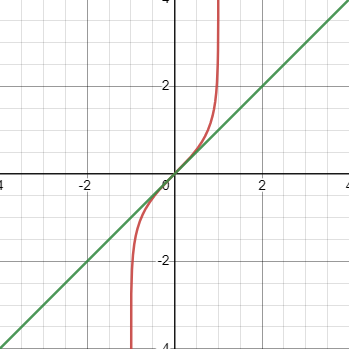
\includegraphics[width=0.4\linewidth]{p1.jpg}
	\end{figure}
	
\end{frame}

\begin{frame}{Solution to a$)$}
	Due to $\left( \mathrm{tanh}^{-1} m \right) \prime=1/(1-m^2)$, we know that $T\ \mathrm{tanh}^{-1}m$ develops a slope of $T$ at the origin. So when $k=Jn \in (0, T\ ]$, $h \in \mathbb{R}$, the two curves intersect at only one point.
	% 由于$\left( \mathrm{tanh}^{-1} m \right) \prime=1/(1-m^2)$,我们知道$T\ \mathrm{tanh}^{-1}m$在原点处的斜率为$T$。所以当$k=Jn \in (0, T\ ]$,$h \in \mathbb{R}$时,两条曲线只在一个点相交。
	\begin{figure}
		\centering
		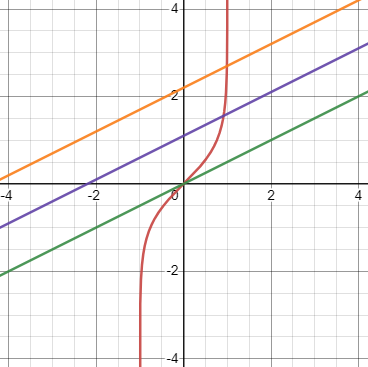
\includegraphics[width=0.4\linewidth]{p2.jpg}
	\end{figure}
\end{frame}

\begin{frame}{Solution to a$)$}
	When $k=Jn > T$, there are one, two, or three solutions depending on the values depending on $h$.
	% 当$k=Jn > T$时,根据$h$的值,有一、两个或三个解。
	\begin{figure}
		\centering
		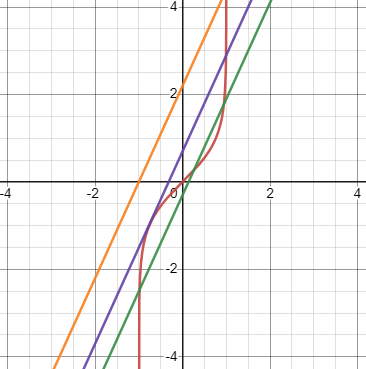
\includegraphics[width=0.4\linewidth]{p3.jpg}
	\end{figure}
\end{frame}

\begin{frame}{Solution to b$)$}
	For the special case $h = 0$, find the critical temperature $T_c$ at which a phase transition occurs.
	% 对于特殊情况$h = 0$,找到发生相变的临界温度$T_c$
	\begin{itemize}
		\item If $h = 0$ and the phase transition occurs when the slope of the line $k=Jn=T$, so the critical temperature is $T_c = Jn$.
		% 如果$h = 0$,且当直线$k=Jn=T$的斜率时发生相变,所以临界温度为$T_c = Jn$
	\end{itemize}
	
\end{frame}

\begin{frame}
	\LARGE \centering Thank you for listening!
\end{frame}

\end{document}

